% Preamble
% ---
\documentclass[a4paper]{article}

% Packages
% ---
\usepackage{bm}
\usepackage[spanish,es-nodecimaldot]{babel}
\usepackage[utf8]{inputenc}
\usepackage[T1]{fontenc}
\usepackage{parskip}
\usepackage{fancyhdr}
\usepackage{mathtools}
\usepackage{amsmath}
\usepackage[htt]{hyphenat}
\usepackage{capt-of}
\usepackage{graphicx}
\graphicspath{ {./images/} }

% Pagestyles
% ---
\pagestyle{fancy}
\rhead{Roselló Beneitez, N. U.; Roselló Oviedo, M.}
\lhead{APR: Práctica sobre SVM}
\fancyfoot[C]{\thepage}

% Main
% ---
\begin{document}

\author{Roselló Beneitez, N. U.; Roselló Oviedo, M.}
\title{APR: Práctica sobre SVM}
\date{6 de Enero de 2020}
\maketitle{}
\thispagestyle{empty}

\newpage
\tableofcontents
\listoffigures

\newpage
\section{Descripción de la práctica}
\quad En esta práctica se han trabajado con máquinas de vector soporte implementadas en Octave mediante la librería \textit{libsvm}. Dicha librería admite diversos  tipos de parámetros, como pueden ser: la tolerancia del sistema modelada mediante el parámetro \textit{C}, el tipo del \textit{kernel} y su grado, entre otras opciones. Los experimentos de esta práctica se han centrado mayoritariamente en pruebas con variaciones de los tres parámetros mencionados previamente, puesto que se considera que son los más relevantes dado lo visto en las sesiones de teoría para la correcta realización de la práctica.

\quad Puesto que las fórmulas utilizadas se encuentran al final de la práctica, se procederá directamente a la exposición de los resultados sin entrar en mayor detalle en el desarrollo matemático de estos.

\section{Un pequeño ejercicio completo de aprendizaje}
\quad En el primer ejercicio a entregar, se han probado diversas combinaciones para los valores de \textit{C} con respecto a los datos linealmente separables y a los no linealmente separables dados por el conjunto de datos \textit{mini}. Concretamente, estos valores han seguido una especie de función logarítmica con el fin de ver el orden de magnitud en el cual los modelos mostraban sus mejores comportamientos.

En primer lugar, para el conjunto separable:

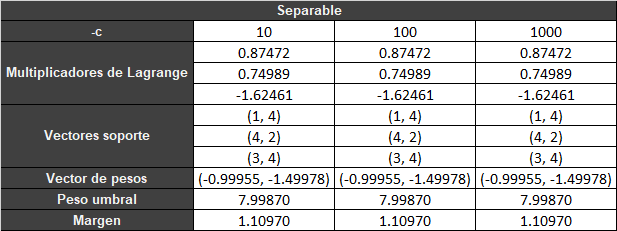
\includegraphics[width=\textwidth]{2_Separables}
\captionof{figure}{Resultados para el conjunto linealmente separable}

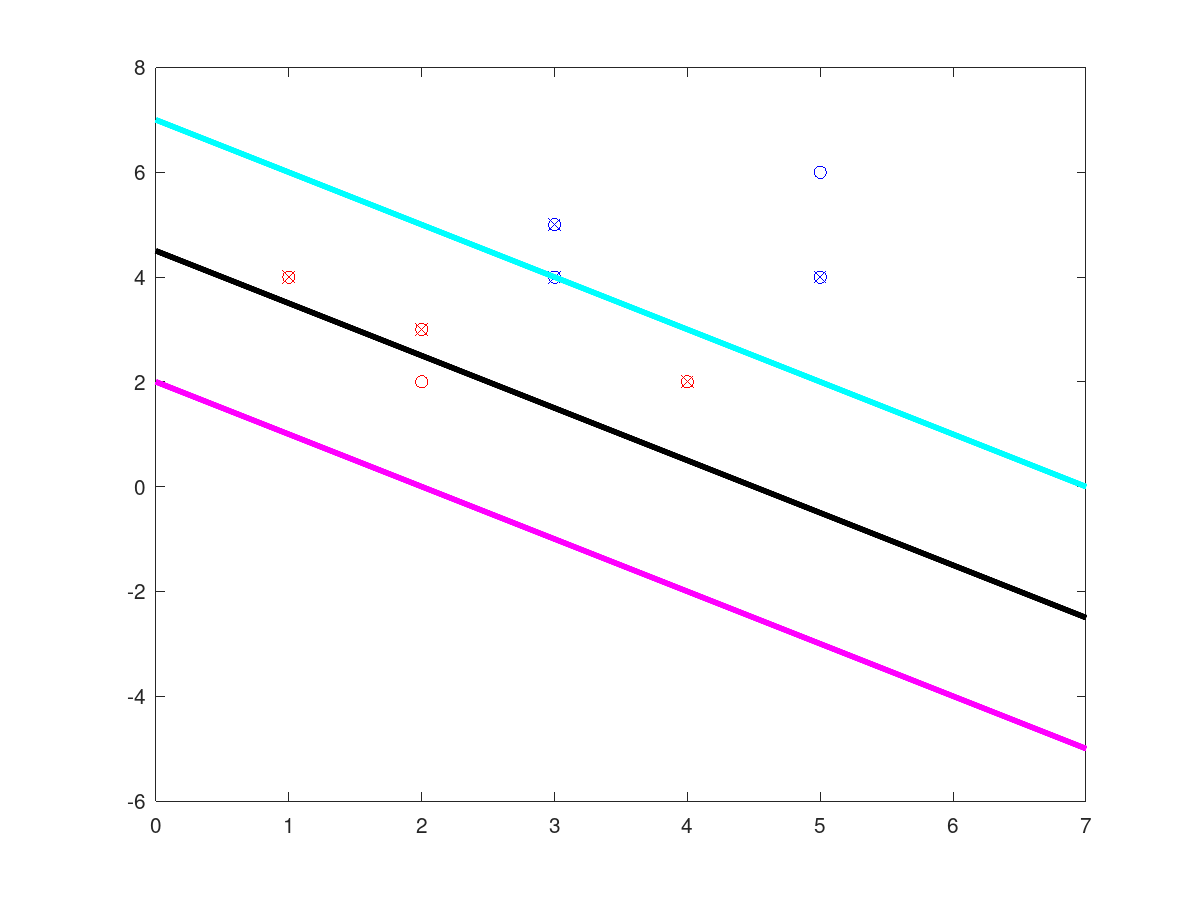
\includegraphics[width=\textwidth]{2_S_01}
\captionof{figure}{Conjunto separable, C = 0.1}

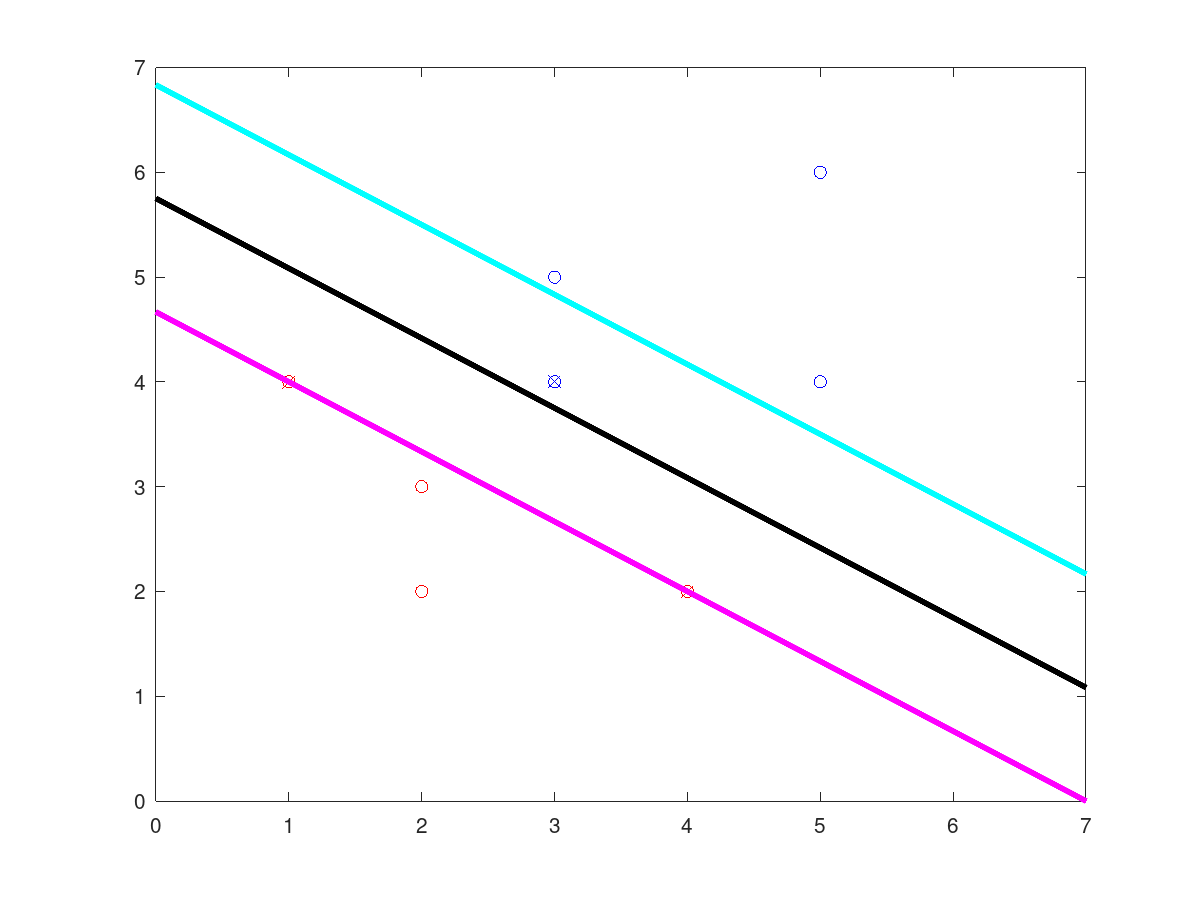
\includegraphics[width=\textwidth]{2_S_1}
\captionof{figure}{Conjunto separable, C = 1}

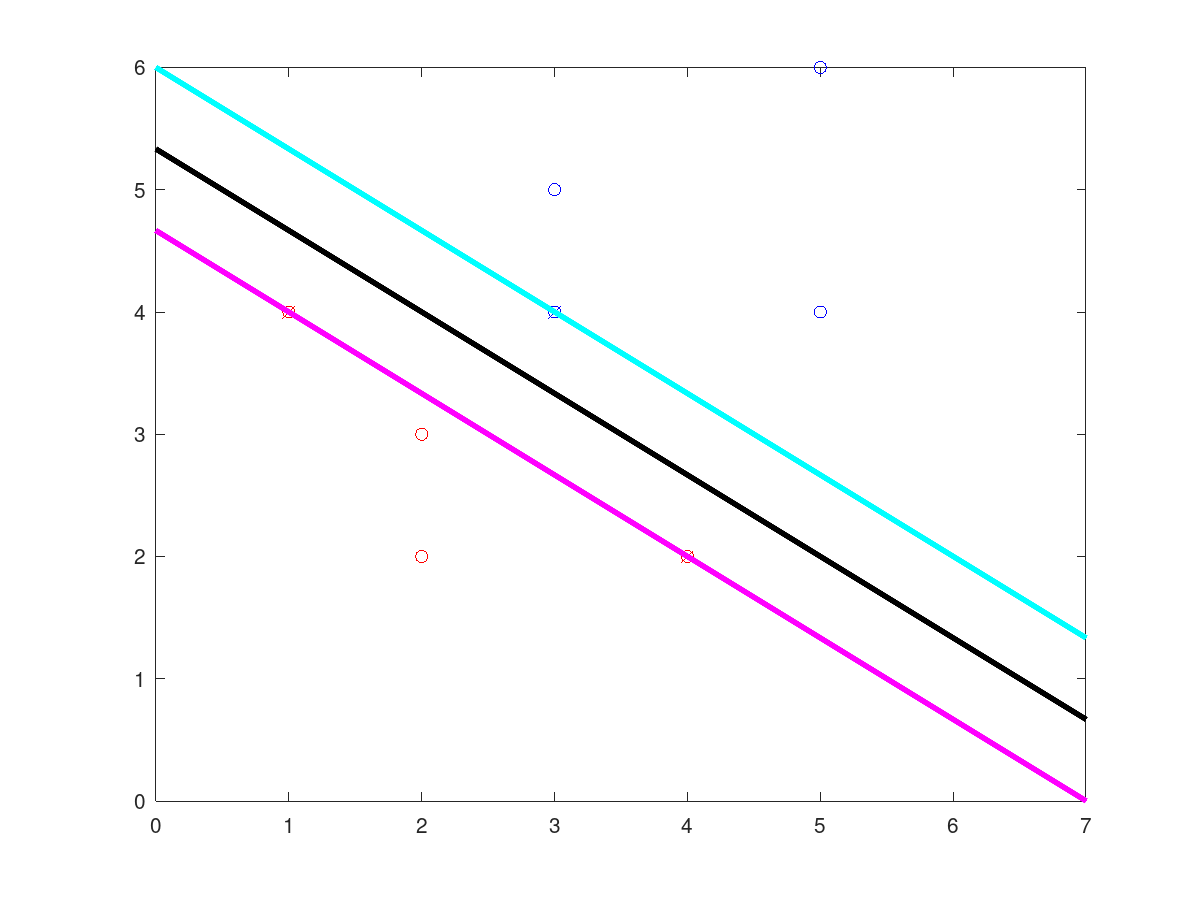
\includegraphics[width=\textwidth]{2_S_10}
\captionof{figure}{Conjunto separable, C = 10}

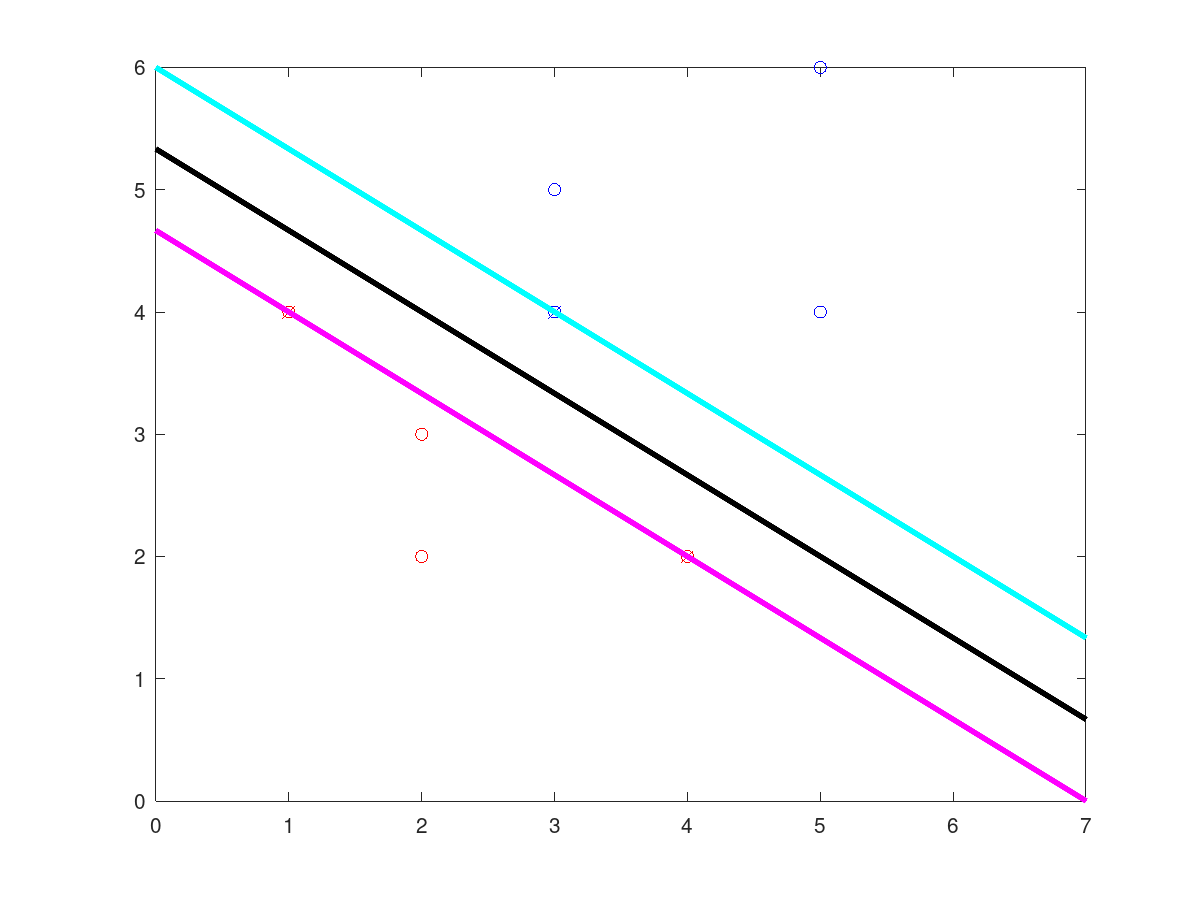
\includegraphics[width=\textwidth]{2_S_1000}
\captionof{figure}{Conjunto separable, C = 1000}
\newpage
En cuanto al conjunto no separable, se ha obtenido:

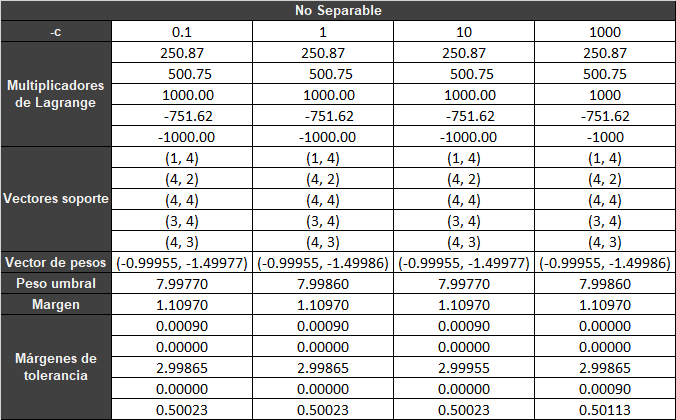
\includegraphics[width=\textwidth]{2_NoSeparables}
\captionof{figure}{Resultados para el conjunto no linealmente separable}

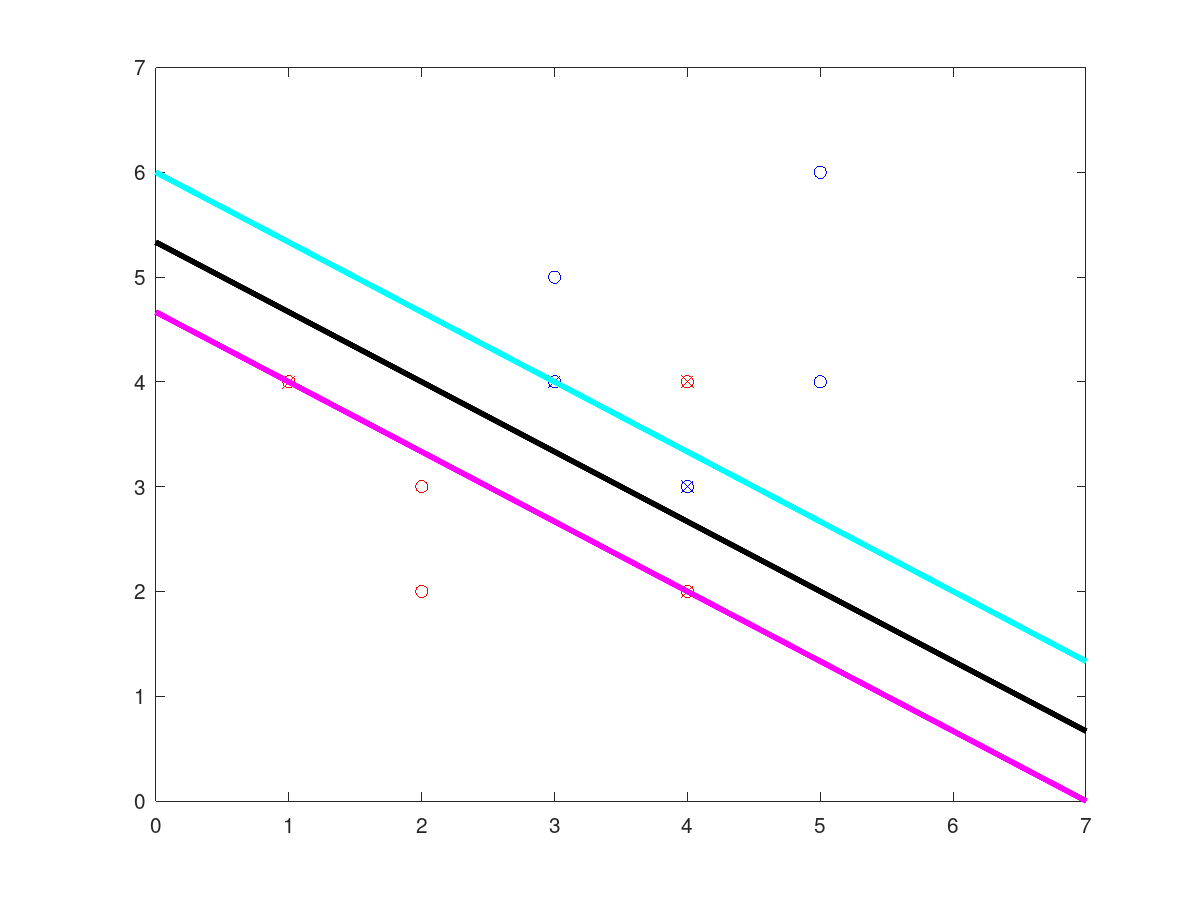
\includegraphics[width=\textwidth]{2_NS_01}
\captionof{figure}{Conjunto no separable, C = 0.1}

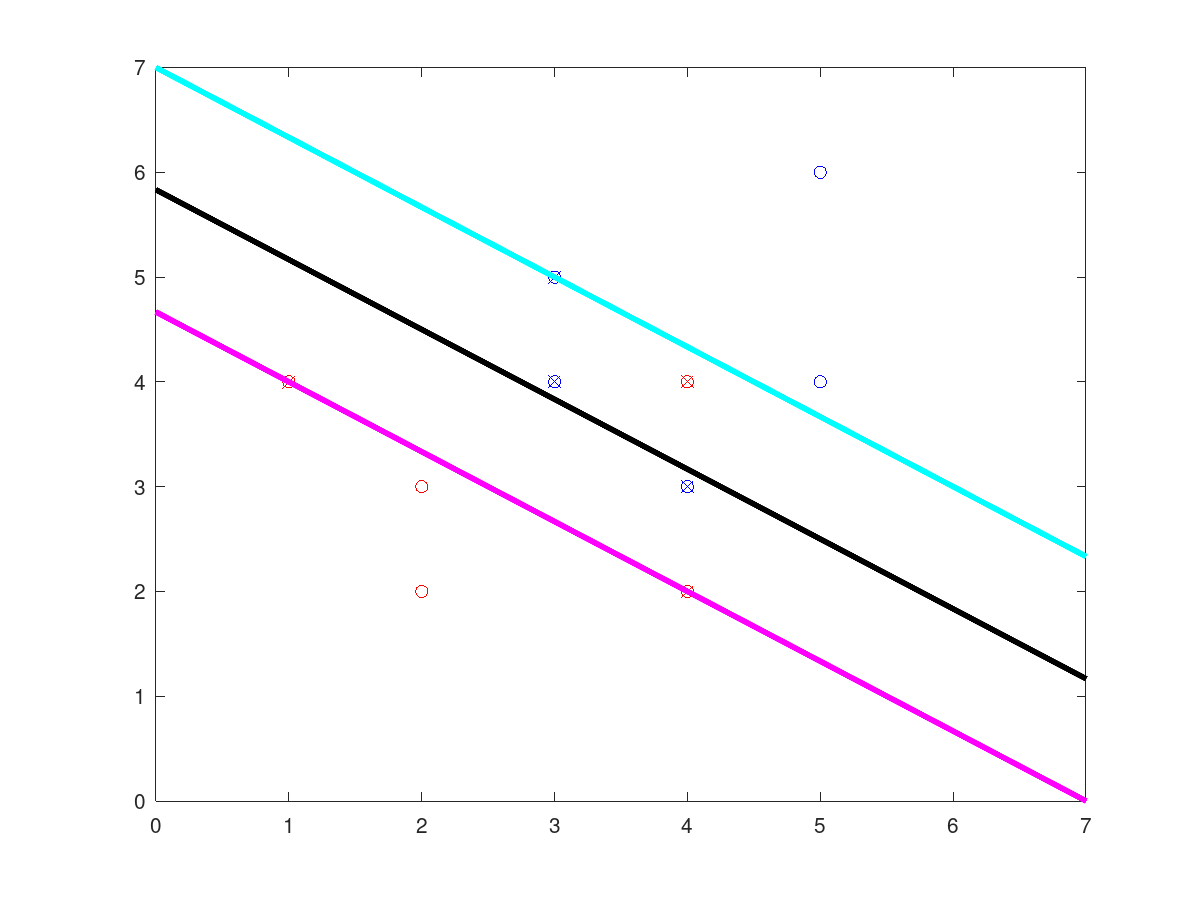
\includegraphics[width=\textwidth]{2_NS_1}
\captionof{figure}{Conjunto no separable, C = 1}

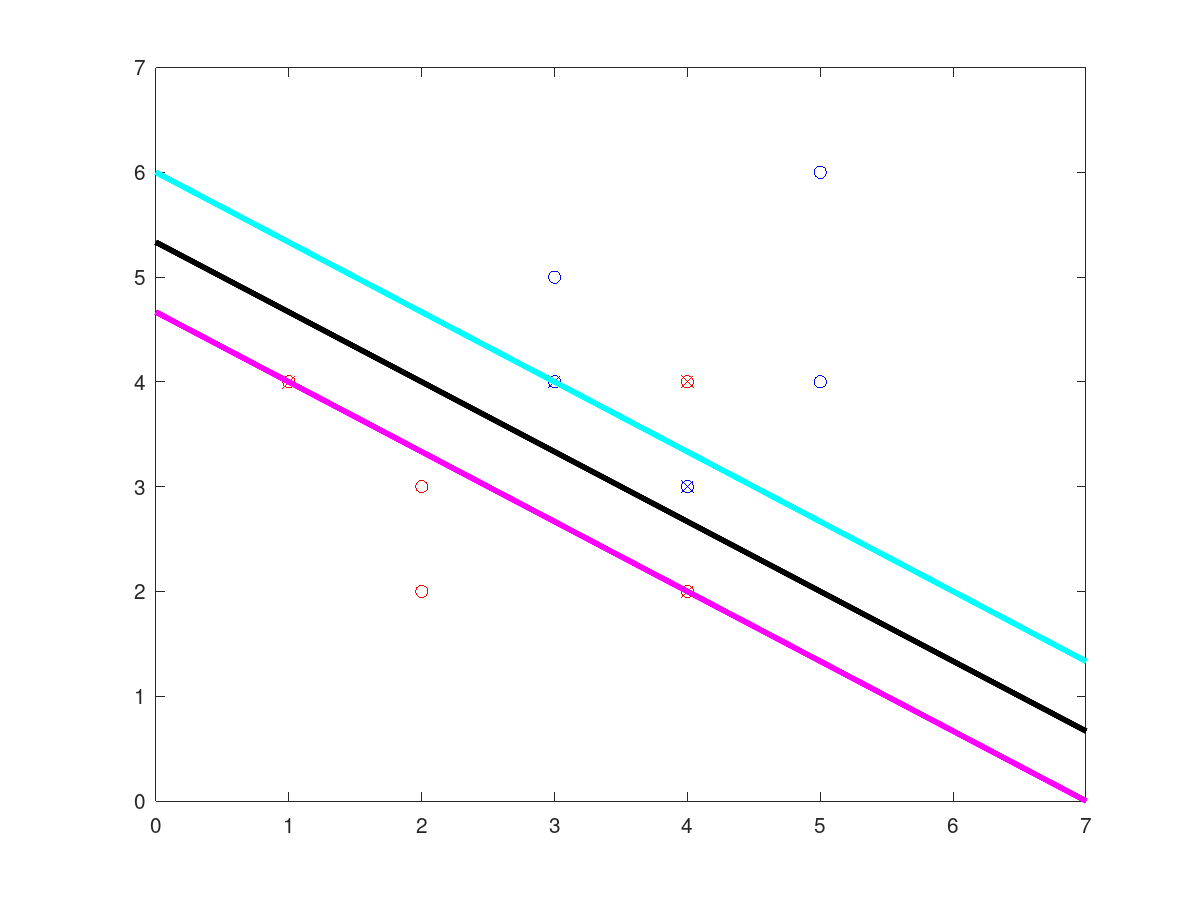
\includegraphics[width=\textwidth]{2_NS_10}
\captionof{figure}{Conjunto no separable, C = 10}

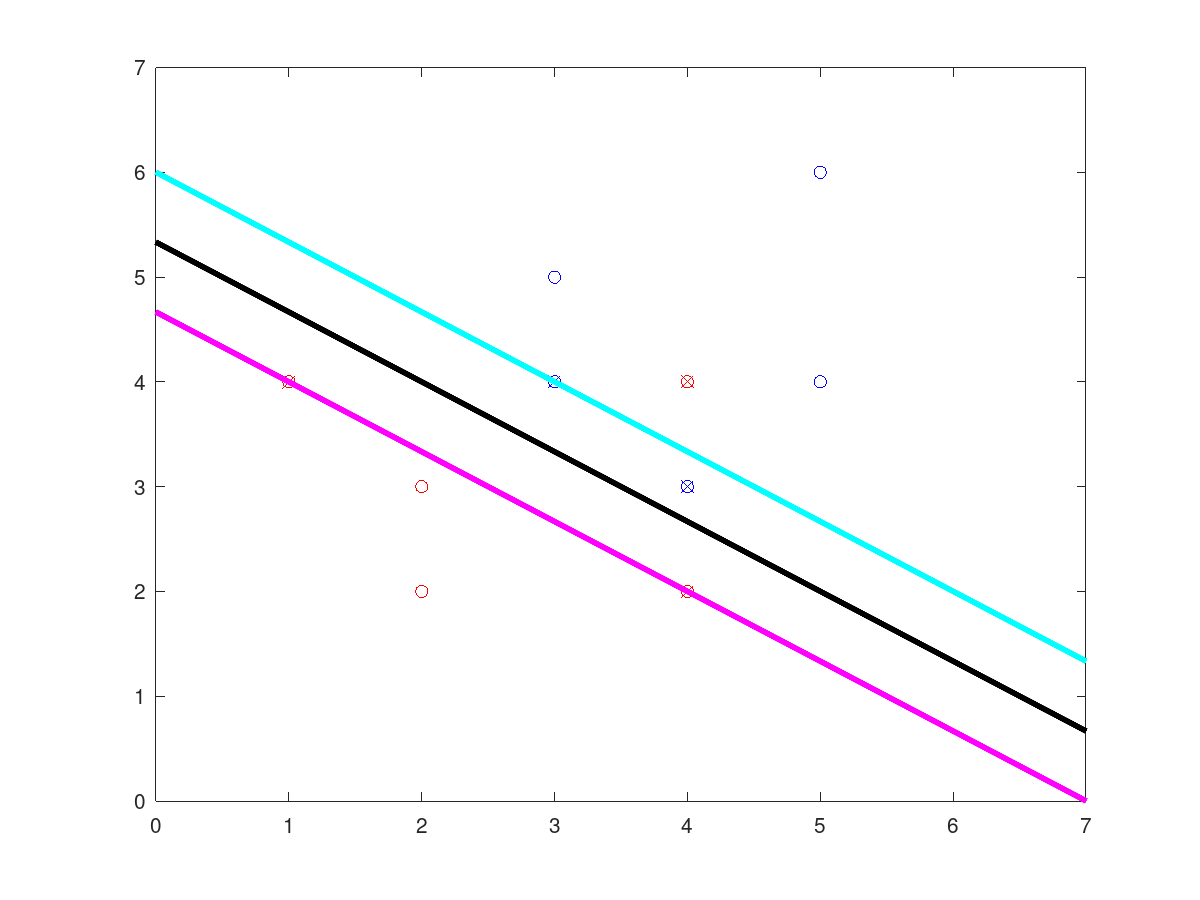
\includegraphics[width=\textwidth]{2_NS_1000}
\captionof{figure}{Conjunto no separable, C = 1000}

\section{Aplicación de SVM a MNIST}
\quad En el segundo ejercicio, correspondiente a la base de datos MNIST, se han probado tanto diversos valores de \textit{C} como diversos grados del polinomio correspondiente al \textit{kernel} con el que se ha ejecutado el entrenamiento. Cabe destacar que únicamente se ha probado este \textit{kernel} polinómico debido a que los otros tipos de kernel disponibles (lineal, gaussiano o de función radial y sigmoide) ya han sido testeados en el entregable de teoría correspondiente al tema 4 y se ha observado como  su tasa de acierto es muy reducida para este caso concreto. Además, se conoce que el \textit{kernel} polinómico es el de mayor acierto gracias a la página web del MNIST. Tras diversas pruebas, se ha determinado que el valor de \textit{C} no es relevante para este caso de estudio, ya que se obtienen los mismos resultados para tolerancias en el rango $\left[ 0.001-1000 \right]$.

\begin{center}
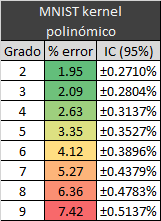
\includegraphics[width=100px]{2_mnist}
\captionof{figure}{Error según el grado del kernel polinómico (MNIST)}

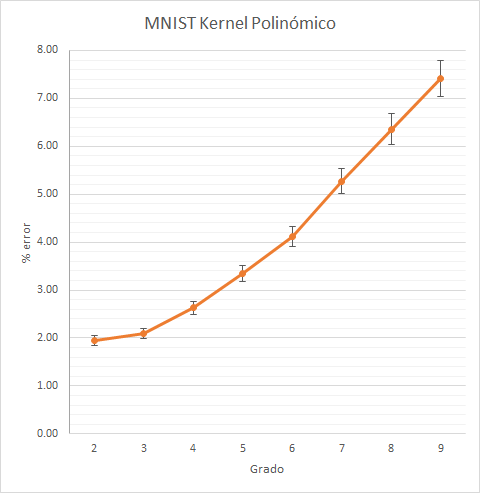
\includegraphics[width=280px]{2_mnist_plot}
\captionof{figure}{Error según el grado del kernel polinómico (MNIST)}
\end{center}

\section{Conclusiones}
\quad Resulta interesante observar el efecto de la tolerancia (\textit{C}) en las muestras linealmente separables y no linealmente separables (ejercicio 3). Este parámetro es similar al parámetro \textit{b} (margen) del \textit{perceptron}: cuanta más \textit{C}, más tienden los parámetros a ser los “correctos”, es decir, los más generalizables. Esto es porque con un valor alto de \textit{C} se premia la minimización de la tolerancia de margen, pero siempre respetando la restricción genérica de las máquinas de vector soporte de que las muestras cuyos multiplicadores de Lagrange no sean 0 estén a una distancia mínima del hiperplano separador.

\quad Cabe mencionar también que, cuando \textit{C} tiende a infinito, se puede observar que la tolerancia de margen de los datos no linealmente separables tiende a ser idéntica a la de los datos linealmente separables. Sin embargo, un valor excesivamente alto de C acaba siendo de poca utilidad debido a que ya no es posible minimizar más la tolerancia de margen; para \textit{C = 10} y \textit{C = 1000} se ha comprobado que los resultados son prácticamente idénticos (excepto los multiplicadores de Lagrange, que se tienen que adaptar al cambio en la \textit{C}).

\quad En cuanto a la base de datos de dígitos MNIST, como se ha podido comprobar en la sección de resultados, el valor de \textit{C} es irrelevante en la medición del error. Esto puede ser debido a que, dado cualquier kernel polinómico de grado mayor o igual a dos, las muestras son polinómicamente separables.

\end{document}
